\subsection{Bedienung}
Die Software zur Bedienung wurde in drei Teile gestaltet. Hardwaremäßig wurde nur das geringste an Elementen verwendet. Die drei Bedienelemente sind jeweils Aktiv High am Mikrocontroller geschaltet mittels einem Taster-Pull-Up-Schaltkreis \ref{fig:SwitchPullUp_Software}. Der Pull-Up Widerstand ist $10k\Omega$, der mit einem Taster auf Erde verbunden wird.

\begin{figure}[h]
	\centering
		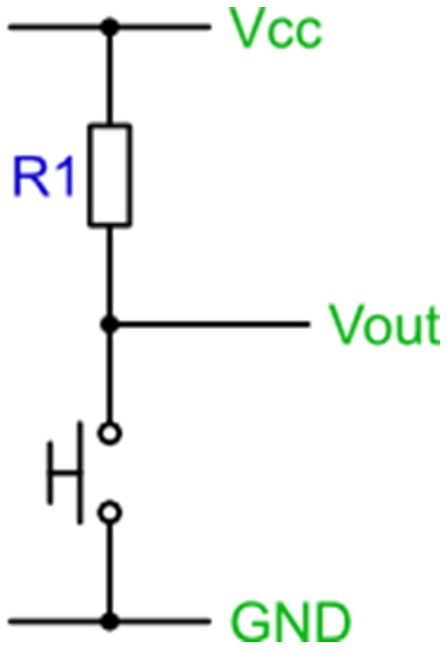
\includegraphics[width=0.25\textwidth]{switchpullupcircuit.jpg}
	\caption{Taster-Pull-Up-Schaltkreis}
	\label{fig:SwitchPullUp_Software}
\end{figure}


%ISR (TIMER0_OVF_vect)
Der Timer-Interrupt im Mikrocontroller ruft alle 16ms eine Funktion auf, die den Taster entprellt, aber auch die Länge des Tasterzustandes registriert.
%button |= ~old_button & current_button & BUTTONMASK;
Der Taster (button) wird als gedrückt erkannt, wenn die Inverse vom alten Zustand (old\_button), dem momentanen Zustand (current\_button) und der Pinmaske (BUTTONMASK)übereinstimmen.
%if (button)
Die folgende If-Bedingung zählt den Bestrahlungswert hoch. Einmal tippen zählt den Bestrahlungswert um eins hoch. Der Wertebereich liegt zwischen 20 und 100. Eine weitere If-Bedingung setzt den Bestrahlungswert beim überschreiten von 100 (Wert grösser gleich 101) zurück auf 20. In dieser sowie in der anderen Bedingung wird das automatische Zählen (autorepeat) auf 50, als Verzögerung, gesetzt.
Der gleiche Code wurde für das Abwärtzählen geschrieben mit dem Unterschied, dass eine Bedingung die Nicht-Zehnerzahlen erkennt und auf die nächst kleinere Zehnerzahl dekrementiert. Würde nämlich die Zahl 55, die ein Integer ist, durch Zehn dividiert mit Zehn multipliziert und um Zehn verringert werden, 40 ergeben.
In der Else-Bedingung wird zunächst geprüft, ob der Taster immer noch gedrückt wird (current\_button and BUTTONMASK). Ist die Bedingung erfüllt, dekrementiert die Funktion einen Wert, der den Unterschied zwischen Tippen und Drücken macht. Bei Null ist die Bedingung erfüllt und der Bestrahlungswert wird um zehn erhöht. Dabei springt er nur auf die nächste Zehnerzahl (Bestrahlungswert gleich Bestrahlungswert geteilt durch 10 multipliziert mit 10 und addiert mit 10). Hier wird wieder darauf geachtet, dass die Zahl 101 nicht überschreitet, sonst wird sie auf 20 zurückgesetzt.
Abgeschlossen wird die Funktion mit dem setzen vom alten Zustand gleich zum neuen Zustand.
Der Bestrahlungswert wird nach der Funktion in eine Variable gespeichert und auf dem Display angezeigt.
\newline